% Default mode is landscape, which is what we want, however dvips and
% a0poster do not quite do the right thing, so we end up with text in
% landscape style (wide and short) down a portrait page (narrow and
% long). Printing this onto the a0 printer chops the right hand edge.
% However, 'psnup' can save the day, reorienting the text so that the
% poster prints lengthways down an a0 portrait bounding box.
%
% 'psnup -w85cm -h119cm -f poster_from_dvips.ps poster_in_landscape.ps'

\documentclass[a0]{a0poster}
% You might find the 'draft' option to a0 poster useful if you have
% lots of graphics, because they can take some time to process and
% display. (\documentclass[a0,draft]{a0poster})

\pagestyle{empty}
\renewcommand{\d}{\mathrm{d}}
\newcommand{\sgn}[1]{\mathop{\mathrm{sgn}}#1}
\newcommand{\bu}{\mathbf{u}}
\newcommand{\bx}{\mathbf{x}}
\newcommand{\br}{\mathbf{r}}
\newcommand{\ds}{\mathrm{d}s}
\newcommand{\ie}{\textit{i.e.}}
\setcounter{secnumdepth}{0}
\newcommand{\comment}[1]{}
\newtheorem{thm}{Theorem}
\newtheorem{prop}{Proposition} 
\newtheorem{corollary}{Corollary} 
\newtheorem{lemma}{Lemma} 
\newtheorem{definition}{Definition}
\newtheorem{example}{Example} 

% The textpos package is necessary to position textblocks at arbitary 
% places on the page.
\usepackage[absolute]{textpos}

% Graphics to include graphics. Times is nice on posters, but you
% might want to switch it off and go for CMR fonts.
\usepackage[final]{graphicx}
\usepackage{wrapfig,helvet}
\usepackage{amsmath}

%to write complex numbers, integers, rationals
\usepackage{amsfonts}
\usepackage{caption}

% These colours are tried and tested for titles and headers. Don't
% over use color!
\usepackage{color}
\definecolor{DarkBlue}{rgb}{0.1,0.1,0.5}
\definecolor{Red}{rgb}{0.9,0.0,0.1}
\definecolor{headingcol}{rgb}{0.5,0.7,1}
%\definecolor{boxcol}{rgb}{0.3,0.8,0.1}

% see documentation for a0poster class for the size options here
\let\Textsize\normalsize
\def\Head#1{\noindent\hbox to \hsize{\hfil{\LARGE\color{DarkBlue}\sf #1}}\bigskip}
\def\LHead#1{\noindent{\LARGE\color{DarkBlue}\sf #1}\bigskip}
\def\Subhead#1{\noindent{\large\color{DarkBlue}\sf #1}\bigskip}
\def\Title#1{\noindent{\VeryHuge\color{Red}\bf\sf #1}}

\TPGrid[40mm,40mm]{23}{12}  % 3 cols of width 7 plus 2 gaps width 1

\parindent=0pt
\parskip=0.5\baselineskip

\makeatletter							%Needed to include code in main file
\renewcommand\@maketitle{%
\null									%Sets position marker
{
\color{headingcol}\sffamily\VERYHuge	%Set title font and colour
\@title \par}%
\vskip 0.6em%
{
\color{white}\sffamily\LARGE				%Set author font and colour
\lineskip .5em%
\begin{tabular}[t]{l}%
\@author
\end{tabular}\par}%
\vskip 1cm
\par
}
\makeatother

\title{A mirror symmetry conjecture: \textit{The fundamental group of the \\ Stringy Kähler Moduli Space acts on $D^b(X)$ via spherical twists}}

\author{Michela Barbieri}

\begin{document}
%----------------------------------------------------------------------%
%           Title bar: across all 21 columns                           %
%----------------------------------------------------------------------%
\begin{textblock}{23}(0,0)
\vspace*{-48mm}\hspace*{-42mm}%

\includegraphics{ucl_bar_black.eps}
\begin{minipage}{1191mm}		%Minipage for title contents
\vspace{-20cm}
\maketitle
\end{minipage}
\end{textblock}

%%%%%%%%%%%%%%%%%% Will need to shift all other content down a bit %%%%%

%----------------------------------------------------------------------%
%           First column.                                              %
%----------------------------------------------------------------------%
\begin{textblock}{7}(0, 2.4)
\Head{The B-side: Toric Geometric Invariant Theory}

\sf % Selects sans serif family: part of the UCL corporate image!
We start with algebraic torus $T \cong (\mathbb{C}^*)^r$ acting on a vector space $\mathbb{C}^n$. These actions 
the actions are simple to write out:
$$
(\lambda_1, \dots, \lambda_r) \cdot (z_1, \dots, z_n) = ({\lambda_1}^{q_{11}}{\lambda_2}^{q_{12}}\dots {\lambda_r}^{q_{1r}} z_1, \dots, {\lambda_1}^{q_{n1}}{\lambda_2}^{q_{n2}}\dots {\lambda_r}^{q_{nr}} z_1)
$$
We get an $n \times r$ integer matrix $Q = (q_{ij})$, called the weight matrix. \\
We construct an algebraic variety that parametrises the actions quotients. \textit{Geometric Invariant Theory} (GIT) is the theory that tells \textit{the unstable locus} to throw away before we quotient so that we get a good/geometric quotient \cite{mumford1994geometric}. GIT quotients are often denoted $X // G$.
\begin{example}
  Consider $\mathbb{C}^*$ acting on $\mathbb{C}^2$ linearly, i.e. $\lambda \cdot (x, \, y) = (\lambda x,\, \lambda y)$.
  If we take the quotient space, we see that the orbit of the origin cannot be separated from any other orbit. So we have to remove the origin and as expected, we get  GIT quotient $$ \mathbb{C}^2 // \mathbb{C}^* = \mathbb{C}^2 \ {(0, \, 0)} / \mathbb{C}^* = \mathbb{P}^1$$
  \begin{figure}
    \centering
    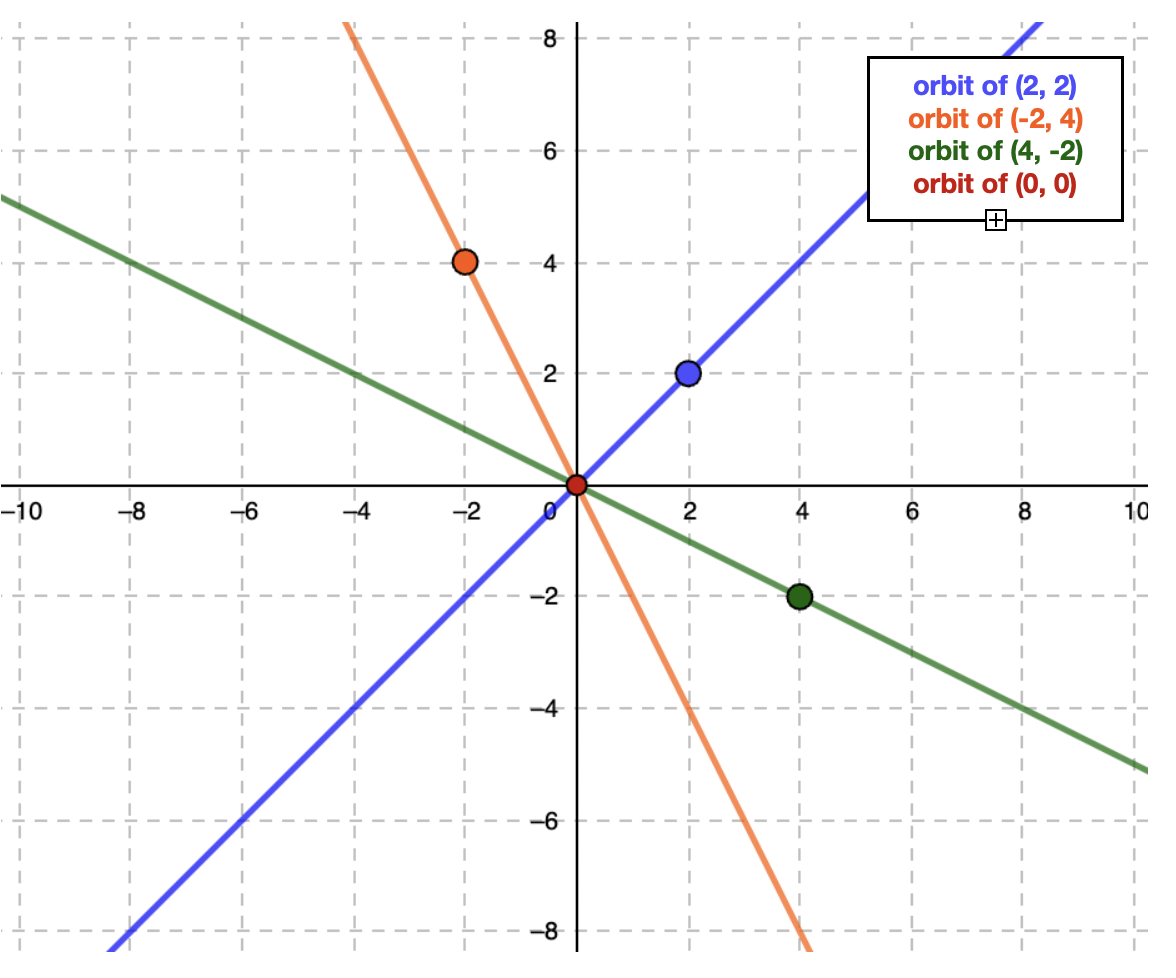
\includegraphics[width=18cm]{orbits of P1.png}
    \caption{Orbits of the $\mathbb{C}^*$ action on $\mathbb{C}^2$.}
  \end{figure}  
\end{example}
In general GIT quotients are not unique and depend on a choice of \textit{stability condition} $\phi \in \mathbb{Z}^r$, where for a given stability condition we denote the GIT quotient $X //_{\phi} G$. Different choices of $\phi$ have us remove different unstable loci and give us non-isomorphic (but birational) quotients.
\begin{example}
  Consider $\mathbb{C}^*$ acting on $\mathbb{C}^3$ via $\lambda \cdot (x, \, y, \, z) = (\lambda x,\, \lambda y, \, \lambda^{-1}z)$. The stability conditions space is $\mathbb{Z}$. For $\phi > 0$, we have unstable locus $Z_{+} = \{ x = y = 0 \}$. We have GIT quotient $$\mathbb{C}^3 //_{\phi} \mathbb{C}^* = \mathbb{C}^3 \backslash{\{ x = y = 0 \}} / \mathbb{C}^* = \mathcal{O}(-1)_{\mathbb{P}^1_{x:y}}.$$
   For $\phi < 0$, we have unstable locus $Z_{-} = \{z = 0\}$.
   $$\mathbb{C}^3 //_{\phi} \mathbb{C}^* = \mathbb{C}^3 \backslash{\{ z = 0 \}} / \mathbb{C}^* = \mathbb{A}^1_{x, \, y}.$$
   \begin{figure}
    \centering
    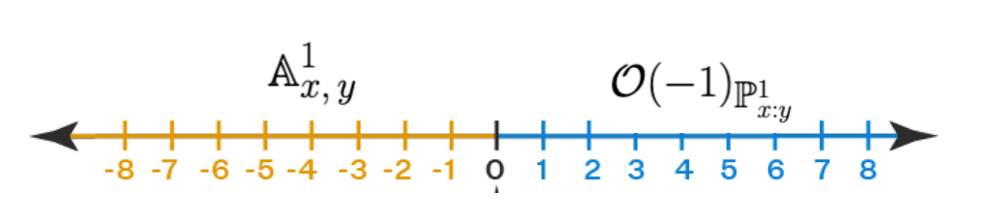
\includegraphics[width=20cm]{diffquotients.png}
    \caption{Secondary fan of GIT problem $\mathbb{C}^3_{(1, \, 1, \, -1 )}$}
  \end{figure}  
\end{example}

\bigskip
\hrule
\end{textblock}

%----------------------------------------------------------------------%
%           Second column.                                             %
%----------------------------------------------------------------------%
\begin{textblock}{7}(8,2.4)
\Head{Mirror Symmetry Conjecture Heuristics}
\sf
Mirror symmetry is a serious of mysterior relationships between complex and symplectic geometry. Its most basic formulation is that given a Kähler manifold $X$, there exists a mirror Kähler manifold $\hat{X}$ such that 
$$
D^b(X) \cong \text{Fuk}(\hat{X})
$$
Actually, we have a whole family of mirrors, each of whom is symplectomorphic to $\hat{X}$, but has a different complex structure. We call the Stringy Kähler moduli space the complex structure moduli space $\mathcal{M}_{CS}$ of the symplectic manifold $\hat{X}$.
\begin{prop}
  There is a monodromy action of $\pi_1(\mathcal{M}_{CS})$ on $\hat{X}$ via symplectomorphism, and hence there is a monodromy action of $\pi_1(\mathcal{M}_{CS})$ on $\text{Fuk}(\hat{X})$ via autoequivalence.
\end{prop}
By mirror symmetry, you expect to be able to carry over the action $\pi_1(\mathcal{M}_{CS})$ to an action of $D^b(X)$ via autoequilvance.
\bigskip
\hrule

\end{textblock}

\begin{textblock}{7}(8,5.4)

\Head{Calabi-Yau Toric GIT}

\sf
Of course, the principal reason for choosing \LaTeX\ is its ability with equations:  
\[ 
   U_\mathrm{doublet} = \frac{mg}{2\pi\mu a}\left( \int_0^\infty \left\{ 1
       - \frac{2\sinh^2{s} - 2s^2}{\sinh{2s}+2s}\right\}\,\ds
   \right)^{-1} \approx \frac{1.55mg}{6\pi\mu a}, \] 
but it's equally easy to include tables: 
\begin{center} 
\begin{tabular}{cccccccccccr}
\hline
  && \multicolumn{2}{c}{$U_1$}  && \multicolumn{2}{c}{$U_2$} 
  && \multicolumn{2}{c}{$U_3$} & $U_3$ \\ 
$L$ &&    MR   &   SD   &&   MR   &   SD   &&   MR    &   SD & error \\ 
\hline
2.01 &&0.65528 &0.64739 &&0.63461 &0.62691 &&0.00498 &0.00451 & 9\%\\ 
2.10 &&0.73857 &0.73126 &&0.59718 &0.58784 &&0.03517 &0.02570 &27\%\\ 
2.50 &&0.87765 &0.87482 &&0.49545 &0.48829 &&0.07393 &0.05853 &21\%\\ 
3.00 &&0.93905 &0.93806 &&0.41694 &0.41356 &&0.07824 &0.06970 &11\%\\ 
4.00 &&0.97964 &0.97945 &&0.31859 &0.31774 &&0.06925 &0.06639 & 4\%\\ 
6.00 &&0.99581 &0.99579 &&0.21586 &0.21575 &&0.05078 &0.05019 & 1\%\\ 
\hline
\end{tabular} 
\end{center}
and, of course, images:
\begin{center}
\rotatebox{-90}{\scalebox{2.22}{\includegraphics{fig2.eps}}}
\end{center}

\bigskip
\hrule
\end{textblock}

%----------------------------------------------------------------------%
%           Third column.                                              %
%----------------------------------------------------------------------%
\begin{textblock}{7}(16,2.4)

\Head{Sectioning}

\Subhead{First Subsection}

\sf
Aenean feugiat, mauris vitae accumsan venenatis, tortor nunc facilisis velit, vel aliquam felis dui non ante. Aenean commodo, sem vel malesuada placerat, erat lacus lacinia magna, quis euismod quam nulla vitae turpis. Vivamus sapien. Vestibulum ante ipsum primis in faucibus orci luctus et ultrices posuere cubilia Curae; Nunc a dolor. Sed diam leo, fringilla non, fermentum non, ultricies tempor, dolor. Mauris vehicula, urna ac bibendum scelerisque, enim nisl vehicula libero, id blandit enim lacus et neque. Nunc posuere elit at erat. Integer commodo, eros dapibus blandit facilisis, dolor ipsum dictum dui, sit amet iaculis enim elit sed magna. Nunc libero nunc, malesuada sit amet, tincidunt at, pharetra ut, arcu.

\bigskip

\Subhead{Second Subsection}

Integer ante. Mauris tincidunt adipiscing mi. Donec sollicitudin, lacus quis pellentesque placerat, quam elit pharetra lacus, sit amet placerat nisi quam in lorem. Etiam id nulla a est vestibulum tempus. Nam et nisl non arcu venenatis semper. Duis sed libero. Cras lectus. In semper urna in leo. Sed mattis lacinia arcu. Phasellus ut metus. Phasellus mi dolor, condimentum ut, ornare nec, tempus ac, mi. Integer ante sem, vestibulum in, gravida vel, condimentum non, ipsum.

\
With the {\tt color} package you can use as much colour as you like: but the \textcolor{Red}{Red} and \textcolor{DarkBlue}{DarkBlue} colours defined here are more useful than the obvious \textcolor{red}{red} and \textcolor{blue}{blue} versions, which tend to seem too bright when printed.

Use spacing as well as colour to highlight a key question or issue: 
\vspace*{1.15\baselineskip}
\begin{center}
\textcolor{Red}{Who will rid me of this turbulent priest?}
\end{center} 
\vspace*{1.15\baselineskip}
Praesent elementum malesuada mauris. Duis aliquet dolor ut nunc. Pellentesque euismod augue a odio. 

\bigskip
\hrule

\bigskip
\end{textblock}


\begin{textblock}{7}(16, 6.35)
\sf
\bibliographystyle{abbrv}
\bibliography{mybib.bib}
\vspace*{4mm} % Sometimes you will have to fudge the final spacing.
\bigskip
\hrule
\end{textblock}

%----------------------------------------------------------------------%
%            Construction lines                                        %

%\begin{textblock}{23}(0,2)\rule{\textwidth}{0.1mm}\end{textblock}
% Shows where the bottom of the header bar should fall.

%\begin{textblock}{23}(0,2.4)\rule{\textwidth}{0.1mm}\end{textblock}
% Shows where the top of each column should start.

%\begin{textblock}{23}(0,12)\rule{\textwidth}{0.1mm}\end{textblock}
% Shows where the bottom of the lowest block in each column should end

%\begin{textblock}{1.5}(6,4.12)\rule{\textwidth}{0.1mm}\end{textblock}
%\begin{textblock}{1.5}(6,4.52)\rule{\textwidth}{0.1mm}\end{textblock}
% Used to find the base of the first block and thus the top of the second.

%\begin{textblock}{1.5}(14,4.85)\rule{\textwidth}{0.1mm}\end{textblock}
%\begin{textblock}{1.5}(14,5.25)\rule{\textwidth}{0.1mm}\end{textblock}
% Same purpose but in the second column.

%\begin{textblock}{1.5}(15,6.05)\rule{\textwidth}{0.1mm}\end{textblock}
%\begin{textblock}{1.5}(15,6.45)\rule{\textwidth}{0.1mm}\end{textblock}
% Same purpose but in the third column.

\end{document}
